\documentclass[11pt]{article}\usepackage[]{graphicx}\usepackage[]{color}
%% maxwidth is the original width if it is less than linewidth
%% otherwise use linewidth (to make sure the graphics do not exceed the margin)
\makeatletter
\def\maxwidth{ %
  \ifdim\Gin@nat@width>\linewidth
    \linewidth
  \else
    \Gin@nat@width
  \fi
}
\makeatother

\definecolor{fgcolor}{rgb}{0.345, 0.345, 0.345}
\newcommand{\hlnum}[1]{\textcolor[rgb]{0.686,0.059,0.569}{#1}}%
\newcommand{\hlstr}[1]{\textcolor[rgb]{0.192,0.494,0.8}{#1}}%
\newcommand{\hlcom}[1]{\textcolor[rgb]{0.678,0.584,0.686}{\textit{#1}}}%
\newcommand{\hlopt}[1]{\textcolor[rgb]{0,0,0}{#1}}%
\newcommand{\hlstd}[1]{\textcolor[rgb]{0.345,0.345,0.345}{#1}}%
\newcommand{\hlkwa}[1]{\textcolor[rgb]{0.161,0.373,0.58}{\textbf{#1}}}%
\newcommand{\hlkwb}[1]{\textcolor[rgb]{0.69,0.353,0.396}{#1}}%
\newcommand{\hlkwc}[1]{\textcolor[rgb]{0.333,0.667,0.333}{#1}}%
\newcommand{\hlkwd}[1]{\textcolor[rgb]{0.737,0.353,0.396}{\textbf{#1}}}%
\let\hlipl\hlkwb

\usepackage{ulem}

\usepackage{framed}
\makeatletter
\newenvironment{kframe}{%
 \def\at@end@of@kframe{}%
 \ifinner\ifhmode%
  \def\at@end@of@kframe{\end{minipage}}%
  \begin{minipage}{\columnwidth}%
 \fi\fi%
 \def\FrameCommand##1{\hskip\@totalleftmargin \hskip-\fboxsep
 \colorbox{shadecolor}{##1}\hskip-\fboxsep
     % There is no \\@totalrightmargin, so:
     \hskip-\linewidth \hskip-\@totalleftmargin \hskip\columnwidth}%
 \MakeFramed {\advance\hsize-\width
   \@totalleftmargin\z@ \linewidth\hsize
   \@setminipage}}%
 {\par\unskip\endMakeFramed%
 \at@end@of@kframe}
\makeatother

\definecolor{shadecolor}{rgb}{.97, .97, .97}
\definecolor{messagecolor}{rgb}{0, 0, 0}
\definecolor{warningcolor}{rgb}{1, 0, 1}
\definecolor{errorcolor}{rgb}{1, 0, 0}
\newenvironment{knitrout}{}{} % an empty environment to be redefined in TeX

\usepackage{xcolor}
\usepackage{alltt}
\usepackage{graphicx, fancyhdr}
\usepackage{amsmath, amsfonts}
\usepackage{color}
\usepackage{hyperref}

\newcommand{\blue}[1]{{\color{blue} #1}}

\setlength{\topmargin}{-.5 in} 
\setlength{\textheight}{9 in}
\setlength{\textwidth}{6.5 in} 
\setlength{\evensidemargin}{0 in}
\setlength{\oddsidemargin}{0 in} 
\setlength{\parindent}{0 in}
\newcommand{\ben}{\begin{enumerate}}
\newcommand{\een}{\end{enumerate}}


\lhead{STAT 305}
\chead{Homework 4} 
\rhead{Sulotion}
\lfoot{Spring 2020} 
\cfoot{\thepage} 
 
\renewcommand{\headrulewidth}{0.4pt} 
\renewcommand{\footrulewidth}{0.4pt} 

\def\Exp#1#2{\ensuremath{#1\times 10^{#2}}}
\def\Case#1#2#3#4{\left\{ \begin{tabular}{cc} #1 & #2 \phantom
{\Big|} \\ #3 & #4 \phantom{\Big|} \end{tabular} \right.}
\IfFileExists{upquote.sty}{\usepackage{upquote}}{}
\usepackage{Sweave}
\begin{document}
\Sconcordance{concordance:stat305-hw4_sol.tex:stat305-hw4_sol.Rnw:%
1 84 1 1 0 16 1 1 9 16 1 1 18 1 1 1 4 1 2 105 1 1 6 45 1 1 5 1 2 2 1 2 %
3 2 1 1 3 1 2 21 1 1 7 9 1 1 6 1 3 1 1 1 2 1 3 22 1}

\pagestyle{fancy} 

Show \textbf{all} of your work on this assignment and answer each question fully in the given context. 

\vspace{0.3cm}

\textbf{If you cannot submit your homework in the class, you can drop it at my office door in 3220 Snedecore Hall by Thursday at 03:30 PM.}

\vspace{0.3cm}

\textcolor{red}{In this homework, you CAN use JMP to plot the data or calculate coefficients of regression model whenever it is asked in the question.}
\vspace{0.3cm}

\emph{Please} staple your assignment and write your name !



\begin{enumerate}



\item
The major cause of axel failure in freight trucks is when shippers exceed the recommended weight limits that can be handled by the axels. 
Issues resulting from these failures have been becoming more frequent as shippers try to cut corners, 
leading members of the state's Department of Transportation to ask one of their civil engineers 
to look into the available data and better advise them on the relationship between excessive weight and axel failure.

A company manufacturing axels provides the engineer with data gathered from conducting experiments loading axels with excessive weight and simulating traveling conditions.
The data consists of two columns, \textbf{excessive weight (in tonnes)} is the amount of weight over the limit that was placed on the axel, and 
\textbf{distance to failure (in tens of thousands of miles)} is the simulated distance to the axel's failure. 

%-- : R code (Code in Document)

\begin{center}
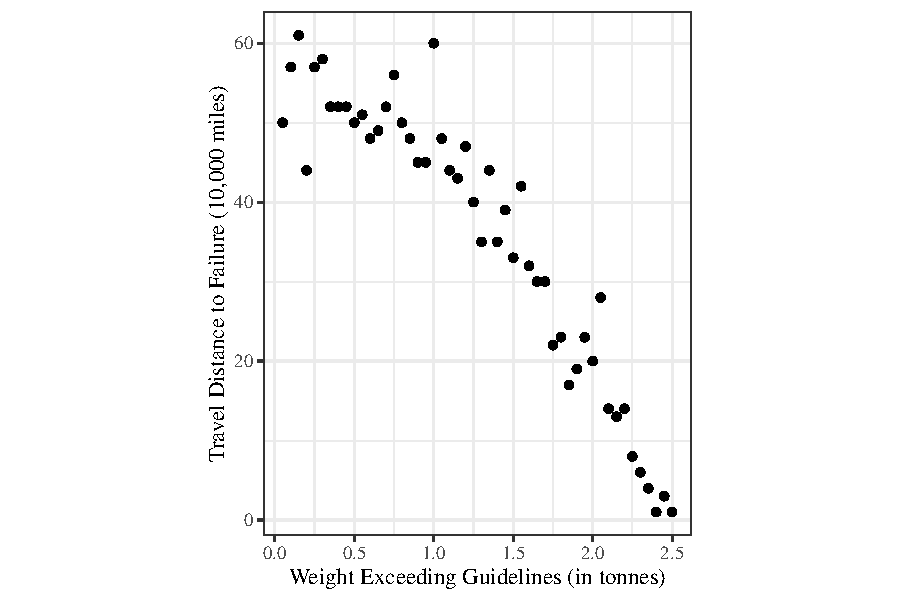
\includegraphics{stat305-hw4_sol-003}
\end{center}

% Here are some summaries of the data:
% 
% $$
% \sum_{i=1}^{50} x_i = 64 \hspace{3cm} \sum_{i=1}^{50} x_i^2 = 107 \\
% $$
% 
% $$
% \sum_{i=1}^{50} y_i = 1795 \hspace{3cm} \sum_{i=1}^{50} y_i^2 = 79777 \\
% $$
% 
% $$
% \sum_{i=1}^{50} x_i y_i = 1699
% $$

\begin{enumerate}
       \item  Using the summaries above, fit a linear relationship between \textbf{weight exceeding guidelines} (x) and \textbf{travel distance to failure} (y).[10 pts]\\
       
        The fitted line equation is 
      $$
      \hat{y} = b_0 + b_1 \cdot x
      $$
      We can use the information above to get the value for $b_1$ and $b_0$:
      \begin{align*}
         b_1 &= \frac{ \sum_{i = 1}^n x_i y_i - n \bar{x} \bar{y} }{ \sum_{i = 1}^n x_i^2 - n \bar{x}^2 } \\
             &= \frac{ (1699) - (50) (64/50) (1795/50) }{ 107 - 50  (64/50)^2 } \\
             &= -23.8676236044657 \\
      \end{align*} 
      and with $b_1$ we can find the value fo $b_0$: 
      \begin{align*}
         b_0 &= \bar{y} - b_1 \bar{x} \\
             &= (1996/50) - (-23.8676236044657)  (64/50) \\
             &= 64.5305582137161 \\
      \end{align*} 

      Which gives us the fitted equation of
      $$
      \hat{y} = 64.53 -23.86 \cdot x
   

      \item Write the equation of the fitted linear relationship. [5 pts] 
      
          \begin{align*}
            \hat{y} = 64.53 -23.86 \cdot x
          \end{align*}
      
      \item Find and \underline{interpret} the value of $R^2$ for the fitted linear relationship.[5 pts]
      
       Since we are using a linear relationship, we can get $R^2$ from $r$ (slides 29 and 51 of chapter 4 slides):
            \begin{align*} 
            r &= \frac{\sum_{i=1}^n x_i y_i - n \bar{x} \bar{y}}{\sqrt{\left(\sum_{i=1}^n x_i^2 - n \bar{x}^2\right)\left(\sum_{i=1}^n y_i^2 - n\bar{y}^2\right)}} \\
              &= \frac{(1982) - (50) (64/50) (1699/50) }{\sqrt{\left(107 - 50 (64/50)^2 \right)\left(94078 - (50)(1699/50)^2\right)}} \\
              &= -0.965183339978807 \\
            \end{align*} 
            So $R^2 = (r)^2 = 0.931578879772645$\\
      
       This means that 93.15\% of our the variablity in travel distance to failure can be explained by the linear relationship with weight exceeding guidelines.
      
      
      \item Using the fitted line, provide a predicted value of travel distance to failure when the weight exceeding the guidelines is 3.4 tonnes.[5 pts]
      
               $$ \hat{y} = 64.53 -23.86(3.4) = -16.594 $$

      \item If the observed travel distance is $0.37$ when the weight exceeding the guidelines is 3.4, what is the residual? Based on the sign of the residual, explain if we are overfitting or under fitting.[5 pts]\\
      

      \emph{Hint:} You have already achieved the predicted value of travel distance when the weight exceeding the guideline is 3.4 in part (d).
      
      
      Using the formula for residuals on page 36-37 of chapter 4 slides, 
            $$ e_{i} = y_i - \hat{y_i}= 0.37 - (-16.594)= 16.964 $$
        The positive residual means that we are  \underline{underpredicting}.    
      
      % \item Sketch what you believe the plot of residuals vs weight would look like. Why would this be a problem?[5 pts]
      % \vspace{2cm}

%
\vspace{0.3cm}
The JMP output below comes from fitting a quadratic model using $x$ and $x^2$.
\vspace{0.3cm}
    
    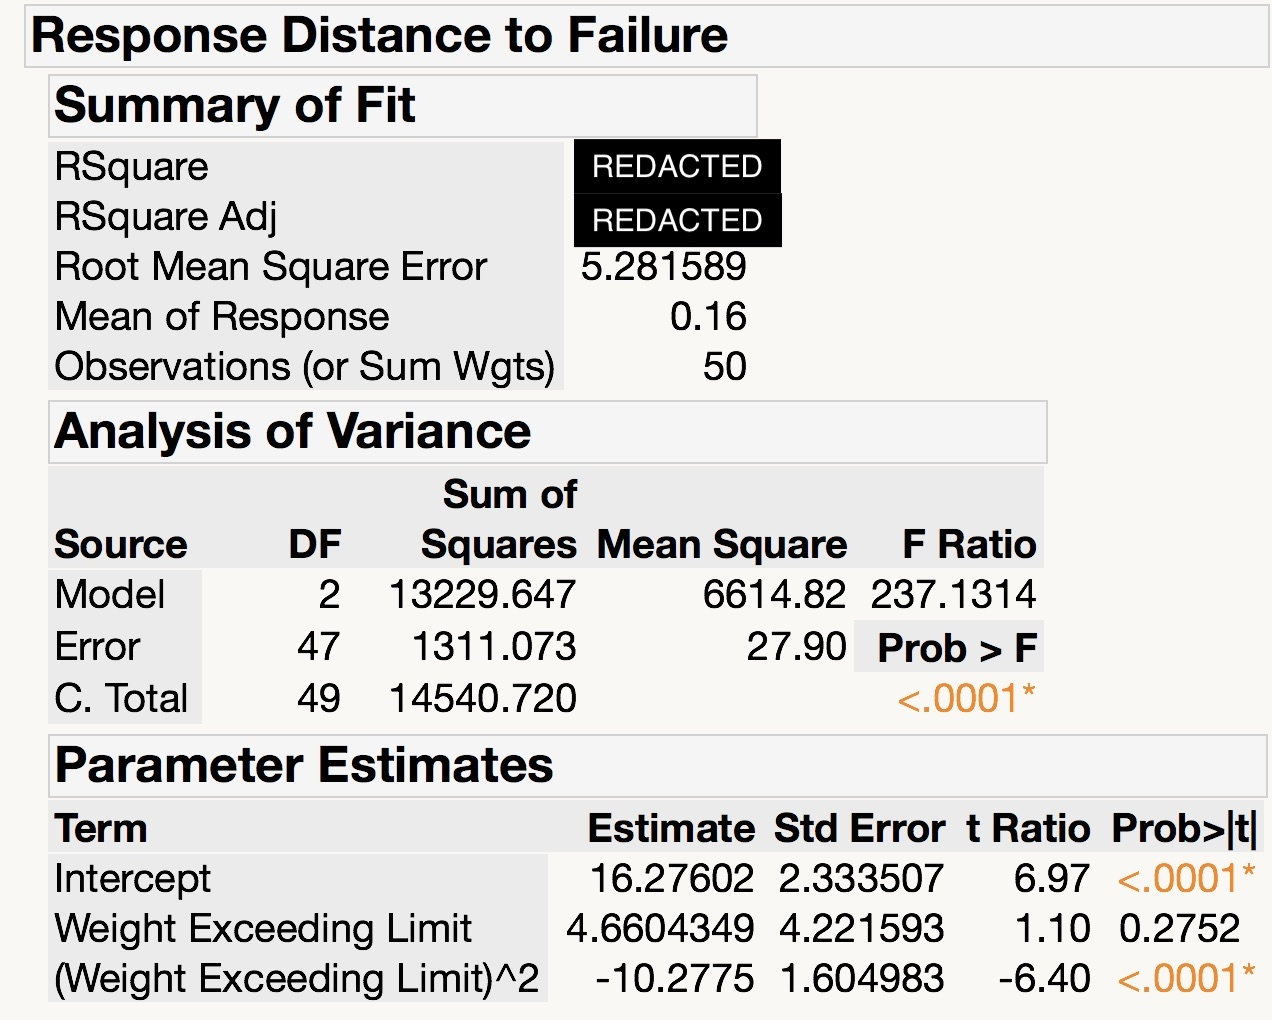
\includegraphics[scale=.2]{FitModel}

\vspace{0.3cm}
       \item Write the equation of the fitted quadratic relationship. [5 pts]
       
             $$\hat{y} = 16.27602 + 4.6604349 x - 10.2775 x^2$$
             
       \item Find and \underline{interpret} the value of $R^2$ for the fitted quadratic relationship.[5 pts]
       
             $$R^2 = 1 - SSE/SSTO = 1 - (1311.073/14540.720) = 0.909834382341452$$
             
      In other words, 90.98\% of the variability in travel distance to failure can be explained by the linear relationship with weight exceeding guidelines.
       
       \item Using the fitted quadratic relationship, provide a predicted value of travel distance to failure when the weight exceeding the guidelines is 3.4 tonnes.[5 pts]

   $$ \hat{y} = 16.27602 + 4.6604349 (3.4) - 10.2775 (3.4)^2 = -86.68640134$$
   
\end{enumerate}




	
	\item \textbf{[Ch. 4.1 Exercise 3, pg. 140]} The article "Polyglycol Modified Poly (Ethylene EtherCarbonate) Polyols by Molecular Weight Advancement" by R. Harris (*Journal of Applied Polymer Science*, 1990) contains some data on the effect of reaction temperature on the molecular weight of resulting poly polyols. The data for eight experimental runs at temperature 165°C and above are as follows (see website for `polyols.csv`):
\begin{center}
\begin{tabular}{r|r}
    \hline
    Pot temperature (°C) & Average molecular weight\\
    \hline
    165 & 808\\
    \hline
    176 & 940\\
    \hline
    188 & 1183\\
    \hline
    205 & 1545\\
    \hline
    220 & 2012\\
    \hline
    235 & 2362\\
    \hline
    250 & 2742\\
    \hline
    260 & 2935\\
    \hline
\end{tabular}
\end{center}
	
Use a statistical package (JMP or `R`) to help you complete the following (plots and computation):

   \begin{enumerate} 
    \item What fraction of the observed raw variation in molecular weight of resulting poly polyols ($y$) is accounted for by a linear equation in reaction temperature ($x$)?[5 pts]\\

Using JMP, the $R^2$ value is 0.9942.
    
    \emph{hint:} The question asks for the coefficient of determination.
    
    \item Fit a linear relationship $y \approx \beta_0 + \beta_1 x$ to these data via least squares. Then explain  how the average mulecular weight changes if pot temperature increases for a $1$°C ?[5pts]
    
    Using JMP, the fitted linear relationship is 
    $$\hat{y}= -3174.6 +23.5 \dot x $$
    
    \item Compute and plot residuals from the linear relationship fit in b). Discuss what they suggest about the appropriateness of that fitted equation.[10 pts]\\
        
    \textbf{Note:} You should provide both residual plots vs. experimental variable and normal QQ-plot vs. residual quantiles to see if the assumptions of the model are met.
    
    
    Using JMP, you can save the residuals of the fit, and then plot residuals vs. experimental variable (reaction temperature) we have 

%-- : R code (Code in Document)
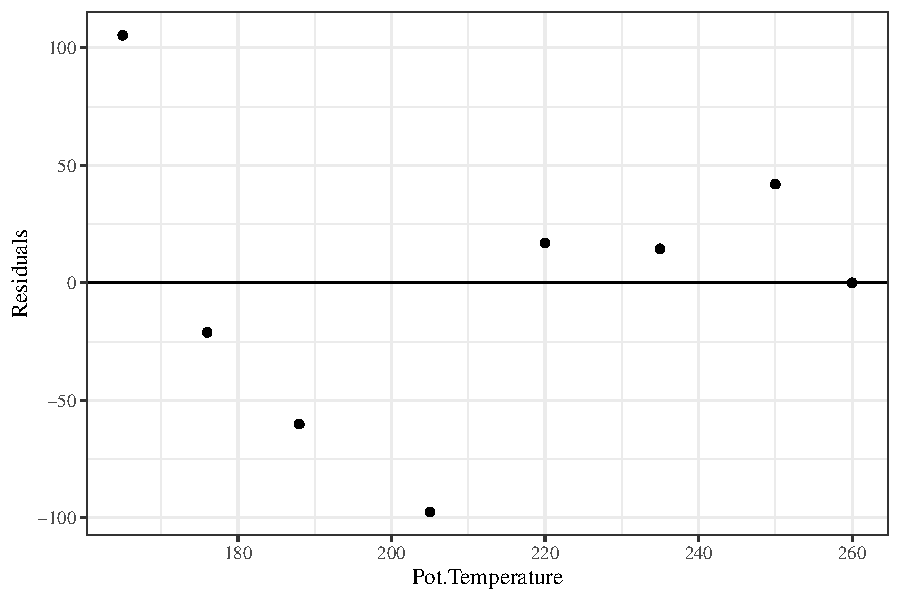
\includegraphics{stat305-hw4_sol-005}
 
 The residual vs. pot temperature plot shows patternless points centered at zero. So, the assumptions of patternless residuals and centered residual at zero seems to be met. To check if the residuals are normally distributed, we can draw a histogram of the residuals and also check normal QQ-plot of residuals. 
 
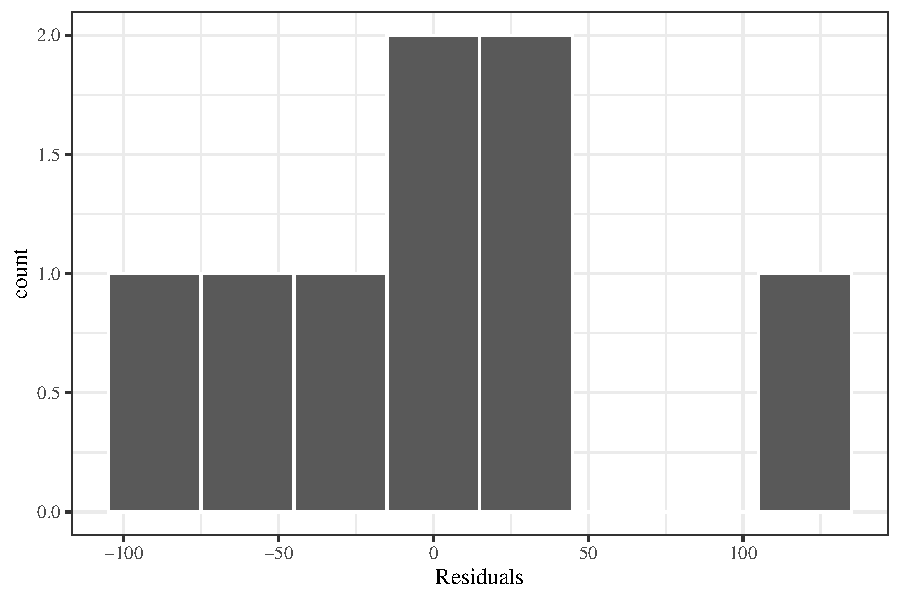
\includegraphics{stat305-hw4_sol-006}
 
    It is hard to evaluate the normality of the residuals based on the  histogram of residuals.  To investigate that more, a better tool is Normal QQ-plot as follow
    
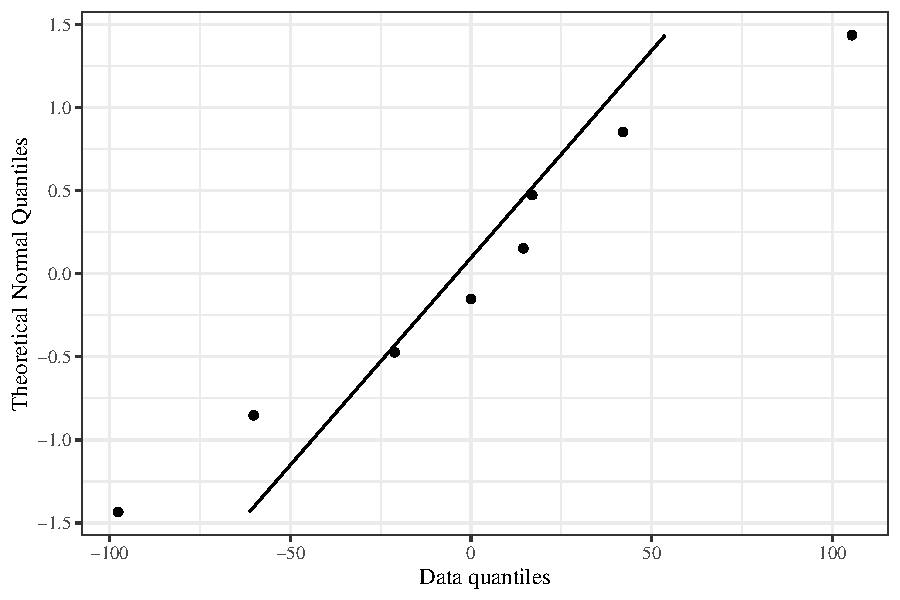
\includegraphics{stat305-hw4_sol-007}
    

 
    The normal qq-plot of residuals is fairly linear, providing no  evidence hat the residuals are not bell shaped. \textbf{So, we can say that the residuals are roughly bell-shaped} and therefore, the assumption of normality is met. 

    \item Based on your analysis of these data, what average molecular weight would you predict for an additional reaction run at $188$°C? At $200$°C? Why would or wouldn't you be willing to make a similar prediction of average molecular weight if the reaction is run at $70$°C?[6 pts]\\
    \emph{Hint:} You may consider extrapolation and/or intrapolation.
	
	for $x= 188$°C 
	$$\hat{y}= -3174.6 +23.5 * (188)= 1243.4 $$
	and for $x= 200$°C, 
	$$\hat{y}= -3174.6 +23.5 * (200)= 1525.4$$
	
	It would not be wise to make a similar prediction at $x=70$°C because there is no evidence that the fitted relationship is correect for pot temeratures as low as $x=70$°C. In other word, that would be extrapolation. some data should be obtained around $x=70$°C before making such prediction. 
	\end{enumerate}

	
	\item  \textbf{[Ch. 4.2, Exercise 1, pg. 161]} Return to problem 2, (Exercise 3 of Section 4.1 on pg. 140 of the textbook). 
	\begin{enumerate}
	
	  \item Fit a quadratic relationship $y \approx \beta_0 + \beta_1 x + \beta_2 x^2$ to the data via least squares.[5 pts] 
	  

	  Using JMP, the quadratic fitted relationship is
	  $$\hat{y}= -1315 + 5.59*x +0.04212*x^2 $$
	  \item Provide the value of $R^2$ and interpret that.[5 pts]
	  
	  Using JMP, the $R^2 = 0.996$ which mneans that 99.6\% of the variation in average molecular weight can be explained by \textbf{the quadratic relationship} between average molecular weight and pot temperature. 
	  
	  \item Plot residuals against the experiemntal variable and normal QQ-plot and discuss if the assumptions of the model are met.[5 pts]
	  
	  
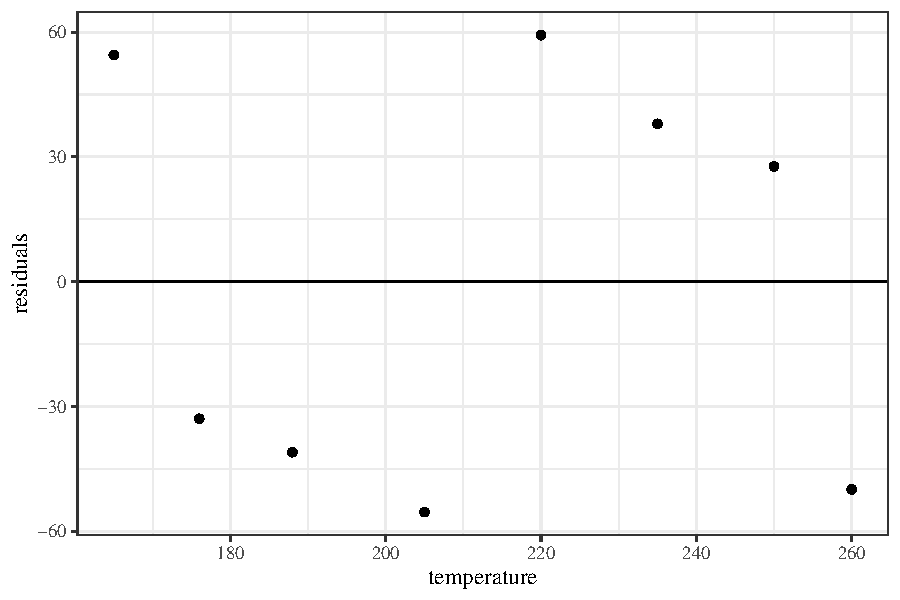
\includegraphics{stat305-hw4_sol-009}


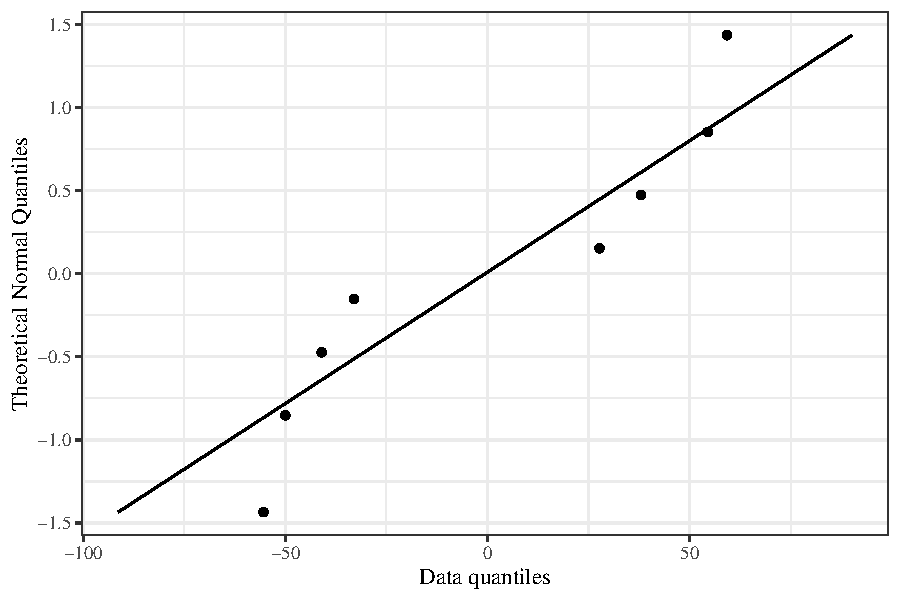
\includegraphics{stat305-hw4_sol-010}

  In general, the residual plots do not show normality of residuals. The residual vs. experimental plot also show some patterned data.   
    
	 The residuals here are smaller, as they will always be more for a more complex model. There is no noticeable improvement in residual plot compared to previous question (fitting a linear line). In fact, the residual plot for the quadratic model looke even more ptterned. 
	 	  

  \end{enumerate}



\end{enumerate}	

Total: 86 pts









\end{document}
